\chapter{He Made \$7M/Year and Paid Zero Taxes!}

These notes follow a School of Hard Knocks interview with Carlton Dennis, arranged here as a companion chapter curated by LazyingArt LLC. The lecture proceeds in a disciplined order, and we should keep that order. First comes the numerical shock; then the legality objection; then the three mechanisms by which the shock is made intelligible; then the practical moves for the earlier operator; then the case studies; and only after all that does the lecture slow down and place an explicit computation on the board. What matters throughout is not merely how much money is earned, but how income is classified, how deductions are created, and how quickly the operator acts before the year closes.

\section{The Opening Puzzle}

The lecture begins with a return to the earlier Ferrari interview. That is not accidental. The car serves as a lure, but the true object is arithmetic. Dennis is reintroduced not merely as a business owner with lifestyle symbols, but as a business owner who claims very high income and very low taxes:

\begin{align}
Y_{2023} &\approx \$7.1\,\text{million}, &
Y_{2024} &\approx \$11.5\,\text{million}, \\
T_{\mathrm{fed},2023} &= \$0, &
T_{\mathrm{state},2023} &= \$26{,}000, \\
T_{\mathrm{total},2024} &< \$92{,}000. &&
\end{align}

This is the lecture's first real move. We are not asked to admire the car; we are asked to confront a paradox. If the income is genuinely at this scale, how can the tax bill remain so small? The host plays his role correctly here. He does not soften the contradiction. He sharpens it.

\subsection{Question \& Answer}

\paragraph{Question.} How can somebody earn millions and still pay almost nothing in taxes without breaking the law?

\paragraph{Answer.} Dennis answers in the language of legality before he answers in the language of technique. He insists that everything is done ``by the book,'' and that the federal side is where he aims to stay near zero, while allowing that California still takes a small share. The lecture then compresses the entire strategy into three recurring devices:
\begin{equation}
\text{tax reduction}
\to
\{\text{income shifting},\ \text{depreciation},\ \text{philanthropy}\}.
\end{equation}
This is the first abstraction of the interview. The puzzle is not resolved by hiding income, but by changing the shape in which taxable income appears and the deductions against which it is measured.

\section{The Three Moving Parts}

Once the legality objection has been met, the lecture names the three operators one by one. Dennis says he focuses on income shifting: how money is moved off the tax return or away from the most expensive line. He focuses on depreciation: how a paper loss can be created through real estate without requiring an equal cash loss in the same period. And he focuses on philanthropy: a private family foundation that contributes outward and reduces the tax bill in the process.

It is important not to flatten this into a list of disconnected hacks. In the lecture it functions as a compact framework. The audience has just heard a shocking number. It now receives a map. The map says that large tax changes do not come from one magic trick. They come from three broad channels, repeated every year and combined in different proportions.

One may summarize the lecture's own compression this way:
\begin{equation}
\text{taxable outcome}
=
\text{income form}
-
\text{allowable deductions}
-
\text{strategic transfers}.
\end{equation}
That is not a statutory formula. It is the structural grammar in which the lecture speaks.

\section{Why Taxes Break the Growing Operator}

At this point the lecture widens from Dennis's own numbers to the ordinary business owner. This is a crucial motivational beat. The host says, in effect, that the point is not only to make money but to keep it. Dennis sharpens the point further: the largest expense for many business owners is not payroll, not the mortgage, and not the car payment. It is taxes.

That matters because the tax bill arrives after the income has already felt liquid. One spends from the bank account as if it were wholly one's own, and only later discovers that some large part of it was already spoken for. In the lecture this is the mechanism by which people go broke. They do not necessarily go broke from lack of revenue; they go broke from spending what should have been reserved for Uncle Sam.

\subsection{Question \& Answer}

\paragraph{Question.} Why do taxes, rather than visible lifestyle expenses, become the real failure point for the growing business owner?

\paragraph{Answer.} Because taxes are a delayed claim on cash. Payroll and rent are paid in the moment and are therefore seen. Taxes accumulate in the background, and for precisely that reason they are easier to ignore. The interview insists that ignorance here is expensive. The operator who has no structure enters the year thinking in gross cash, and exits it owing against money that may already have been consumed.

From there Dennis gives the first strong relief mechanism. If the income is W-2 or 1099 income, then short-term rentals become a candidate machine for creating deductions:
\begin{equation}
\text{cost segregation}
\Rightarrow
\text{paper loss}
\Rightarrow
\text{offset W-2 / 1099 income}.
\end{equation}
The local conditions arrive in practical language, not in legal jargon:
\begin{equation}
\mathrm{STR}=7\ \text{days or less},
\qquad
\text{manage for }100\ \text{hours}.
\end{equation}
The lecture also extends this logic to the household. If one spouse is not otherwise working, then that spouse can, in Dennis's telling, become the real-estate professional who manages the portfolio and strengthens the active-business posture of the real-estate side. In this way the lecture makes a transition from an individual tax problem to a family operating structure.

\section{Beginner Structure Before Big Assets}

The host then performs the right correction. Many viewers are not yet in position to buy the kind of property just described. He places the question in the mouth of the younger operator, even referring to his own company's first seven-figure year, and asks what the person should do when the tax bill is arriving before the real-estate machine is available.

The lecture answers with entity structure. Dennis places the threshold near the point where self-employed income rises past roughly \$50{,}000 to \$60{,}000:
\begin{equation}
I_{\text{self-employed}} \gtrsim \$50{,}000\text{--}\$60{,}000
\Rightarrow
\text{consider S-corporation treatment}.
\end{equation}
The rate that matters in his explanation is
\begin{equation}
\tau_{\mathrm{SE}} = 15.3\%.
\end{equation}
If we write his explanation in cleaned lecture-note form, we obtain
\begin{align}
T_{\mathrm{SE,sole\ prop}} &\approx \tau_{\mathrm{SE}}\Pi, \\
T_{\mathrm{SE,S\ corp}} &\approx \tau_{\mathrm{SE}}S,
\end{align}
where \(\Pi\) denotes business profit and \(S\) the owner's salary. We should read this as a lecture-level model of the point, not as a full derivation of all payroll and self-employment rules. The point is that once a salary is separated from the remaining profit, the tax burden discussed in the interview no longer strikes the whole pool in the same way.

\subsection{Question \& Answer}

\paragraph{Question.} Why does the S-corporation threshold matter once a self-employed person crosses roughly \$50{,}000 to \$60{,}000?

\paragraph{Answer.} Because below that region, simplicity may dominate. Above it, the difference between taxing all profits and taxing only the salary component becomes large enough that legal form itself becomes economically material. The threshold is therefore not a theorem of tax law but a threshold of practical relevance in the lecture's own pedagogy.

The interview then adds a second, far less glamorous, move. Many operators are already spending money on business uses without classifying it properly. Dennis therefore treats deduction recovery as the immediate discipline of the early-stage operator. Expenses paid on a personal card but properly belonging to the business can still be allocated back across the boundary. The lecture gives simple examples:
\begin{itemize}
\item cell phones,
\item laptops,
\item travel that was in fact business travel.
\end{itemize}
There is nothing romantic here, and that is precisely the point. Before one has a large real-estate structure, one still has classification, entity choice, and the accuracy of the accounting line.

\section{Speed, Evidence, and Leverage}

Only after the beginner remedies does the lecture turn to what Dennis calls the difference between middle-class and wealthy behavior. The answer is blunt: speed. The wealthy do not merely ask whether a move is possible. They ask where the money should go, when the foundation should be set up, and where the wire should be sent. It happens, he says, in hours rather than weeks.

This is not merely psychology. It is temporal mechanics. Tax planning is path-dependent. The move that is delayed too long becomes impossible within the relevant year, and what could have been moved into structure ends as a check written in cash.

The host then asks for proof by case. Dennis claims to have saved clients well over \$100 million in taxes, and the lecture next turns to a story of an IRS challenge involving a yacht. The central lesson is documentation. The claimed deduction survives, in Dennis's telling, because the taxpayer can produce records: the captain's log, photographs, and the trail of expenses. He also states the legal standard in words rather than symbols: the expense must be ordinary, necessary, and reasonable in the pursuit of income. It is wise to preserve that standard while not leaning too heavily on the exact code citation named in the transcript, since the transcript's numeric reference is not entirely secure.

The interview then shifts from audit defense to vehicle logic. Here the G-Wagon becomes an explicit tax object. Dennis says the vehicle produced about \$92{,}000 in tax savings, and that those savings were pushed into a multifamily property producing about \$1{,}400 per month in cash flow:
\begin{equation}
\Delta T_{\mathrm{G\text{-}Wagon}} \approx \$92{,}000
\to
\text{multifamily reinvestment}
\to
\$1{,}400/\text{month}.
\end{equation}
He then states the eligibility conditions:
\begin{equation}
\mathrm{GVWR} > 6{,}000\ \text{lb},
\qquad
u_{\mathrm{biz}} > 50\%.
\end{equation}
The lecture names the deduction route as
\begin{equation}
\text{Section }179 + \text{Section }168\mathrm{K},
\end{equation}
and places the vehicle example inside the depreciation timeline
\begin{equation}
b_{2023}=80\%,
\qquad
b_{2024}=60\%.
\end{equation}
Dennis also speculates that bonus depreciation could return to \(100\%\). These notes record that as a lecture-side expectation, not as an assumption needed elsewhere in the chapter.

\subsection{Question \& Answer}

\paragraph{Question.} How can a depreciating asset or a debt-financed purchase still improve the operator's financial position?

\paragraph{Answer.} Because the lecture is comparing cash paths, not merely sticker prices. Dennis's example is deliberately simple:
\begin{align}
I &= \$200{,}000, \\
E_{\mathrm{down}} &= \$20{,}000, \\
W &\approx \$200{,}000, \\
T_{\mathrm{counterfactual}} &\approx \$50{,}000.
\end{align}
If the write-off neutralizes the income, then the interview invites us to compare the tax that would have been paid with the cash used to take control of the vehicle:
\begin{equation}
\$50{,}000 - \$20{,}000 = \$30{,}000.
\end{equation}
The point is not that the car appreciates. The point is that the avoided tax, once redeployed, can dominate the down payment.

From here the lecture widens into leverage in the larger sense. Dennis distinguishes bad debt from good debt:
\begin{equation}
\text{consumer debt}\to \text{bad debt},
\qquad
\text{asset-backed leverage}\to \text{good debt}.
\end{equation}
He then offers two heuristics that should be preserved as heuristics and not elevated into law:
\begin{equation}
L_{\mathrm{loan}}\uparrow \Rightarrow \text{buying power}\uparrow,
\qquad
\text{wealth}\sim \text{access to debt}.
\end{equation}
Real estate is his favorite stage for these heuristics because leverage enlarges the position, HELOCs and cash-out refinances re-release capital, and the resulting portfolio can outlive the debt work that created it. The lecture even pauses on the social technology that makes this possible: use credit, accumulate deposits, build the banking relationship, and eventually obtain the private banker who understands the business model well enough to underwrite larger moves.

Only after that banking aside does the interview come to its cleanest example.

\section{The Board Example: A \$500{,}000 Property and a \$100{,}000 Paper Loss}

The board arrives late, and that timing matters. By the time Dennis begins writing, the audience has already heard the legality defense, the three-part framework, the beginner structures, the speed argument, the audit story, the car logic, and the leverage argument. The whiteboard therefore functions as payoff rather than introduction.

\begin{figure}[h]
\centering

\includegraphics[width=0.82\textwidth]{lecture_56_figure_03.png}
\end{figure}

The screenshot should remain here because the board itself is evidentiary. We can read the short-term-rental condition, the \(100\)-hour management requirement, the cost-segregation label, and the final \(\$100{,}000\) result, although part of the writing is blocked by the gesture and the microphone.

The board's logic can be redrawn in cleaned form without replacing the original evidence:

\begin{figure}[h]
\centering
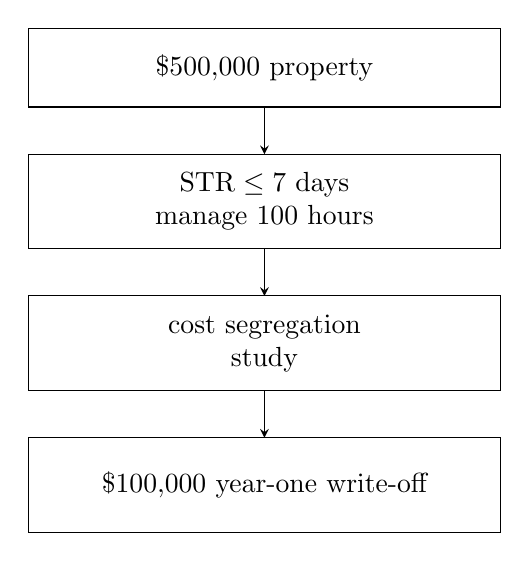
\begin{tikzpicture}[>=stealth]
\draw (-3,6.2) rectangle (3,7.2) node[pos=.5]{\(\$500{,}000\) property};
\draw (-3,4.4) rectangle (3,5.6) node[pos=.5]{\shortstack{\(\mathrm{STR}\le 7\) days\\manage \(100\) hours}};
\draw (-3,2.6) rectangle (3,3.8) node[pos=.5]{\shortstack{cost segregation\\study}};
\draw (-3,0.8) rectangle (3,2.0) node[pos=.5]{\(\$100{,}000\) year-one write-off};
\draw[->] (0,6.2) -- (0,5.6);
\draw[->] (0,4.4) -- (0,3.8);
\draw[->] (0,2.6) -- (0,2.0);
\end{tikzpicture}
\end{figure}

The visible board conditions are worth restating exactly as they appear in cleaned typeset form:
\begin{equation}
\mathrm{STR}=7\ \text{days or less},
\qquad
\text{manage for }100\ \text{hours}.
\end{equation}

\subsection{Question \& Answer}

\paragraph{Question.} How does a \$500{,}000 property become a \$100{,}000 paper loss?

\paragraph{Answer.} Here we should stay very close to the lecture's spoken order.

\begin{enumerate}
\item Start with an operator earning
\[
I_{\mathrm{W2}}=\$100{,}000.
\]

\item Take a property with purchase price
\[
P_{\mathrm{prop}}=\$500{,}000.
\]

\item Finance it with
\[
E_{\mathrm{down}}=\$100{,}000,
\qquad
L_{\mathrm{loan}}=\$400{,}000.
\]

\item Put the property into short-term-rental use and satisfy the lecture's two local conditions:
\[
\mathrm{STR}=7\ \text{days or less},
\qquad
\text{manage for }100\ \text{hours}.
\]

\item Perform a cost segregation study and use the lecture's rule of thumb
\[
W_{1}=20\%\cdot P_{\mathrm{prop}}.
\]

\item Compute the year-one write-off:
\[
W_{1}=0.20\times \$500{,}000=\$100{,}000.
\]

\item Match the paper loss against the original income:
\[
I_{\mathrm{W2}}=\$100{,}000,
\qquad
L_{\mathrm{paper}}=\$100{,}000
\Rightarrow
T\approx 0
\]
in the example as presented.
\end{enumerate}

\paragraph{Caveat.} The board is only partially legible. The \(\$500{,}000\) input and the exact lower expression are not fully visible, so the cleaned equation
\[
0.20\times \$500{,}000=\$100{,}000
\]
should be read as a cautious reconstruction anchored by both the visible board layout and the spoken line that the result ``would equal a hundred thousand.'' The surrounding transcript also contains one stray phrase that sounds like ``a hundred thousand dollar property,'' but the arithmetic before and after it clearly belongs to the \$500{,}000 example.

The lecture then immediately widens the scale. If a \$500{,}000 property can neutralize \$100{,}000 of income under this rule of thumb, then a larger property paired with larger income extends the same percentage logic. That is why Dennis returns once more to debt. The real constraint is not ownership in cash of the whole asset. It is access to enough equity, enough borrowing capacity, and enough structure to turn the asset into a deduction engine.

\section{The Augusta Rule}

The lecture closes with one more move that is smaller than the real-estate example but cleaner in its threshold. Dennis gives the story through Augusta, Georgia, where homeowners rented primary residences during the Masters because the city could not house all visitors. The rule is then condensed to the numerical boundary that matters:
\begin{equation}
d_{\mathrm{Augusta}} \le 14\ \text{days}.
\end{equation}
He names the federal reference in the interview as
\begin{equation}
\mathrm{IRC}\text{-}280\mathrm{A}.
\end{equation}

The form of the rule is simple enough to carry away from the lecture. A primary residence rented for a sufficiently short window can generate rental income that, in Dennis's presentation, is not taxed to the owner. He then folds this back into the S-corporation machinery already introduced earlier.

\subsection{Question \& Answer}

\paragraph{Question.} Why does the Augusta Rule function like a tax-free distribution back to the owner?

\paragraph{Answer.} Because the lecture treats the owner and the S corporation as distinct actors in the transaction. The chain is:
\begin{equation}
\text{owner} \leftrightarrow \text{S corp}
\to
\text{rent residence for }14\text{ days}
\to
\text{deduction at S-corp level + tax-free rent to owner}.
\end{equation}

We may rewrite the lecture's logic as a short sequence:
\begin{enumerate}
\item The owner controls an S corporation.
\item The S corporation rents the owner's primary residence.
\item The rental period stays within the \(14\)-day window.
\item The corporation deducts the rent.
\item The owner receives the rent under the lecture's tax-free treatment of that short rental window.
\end{enumerate}

This is why Dennis presents the rule as low-hanging fruit. It is not the largest machine in the lecture, but it is the cleanest final one: a named rule, a numerical threshold, and a short operational loop from entity to individual.

\section{Summary}

The lecture begins with a paradox and ends with a sequence of lawful mechanisms. First the large income and small tax bill are placed before us. Then the legality objection is voiced and answered. Then the interview compresses itself into three recurring operators: income shifting, depreciation, and philanthropy. After that it slows down and differentiates scales. The wealthy operator gets the large real-estate paper-loss machine; the earlier operator gets entity structure and deduction recovery; the hesitant operator is told that delay itself is costly; and the skeptical operator is shown audit records, vehicle arithmetic, and leverage logic.

The mathematical center of the chapter remains the board example:
\[
0.20\times \$500{,}000=\$100{,}000.
\]
Everything before it prepares the reader to understand why that line matters. Everything after it compresses the lesson into one last portable rule. The lecture's real claim, then, is not mystical. Tax outcomes are shaped by classification, depreciation, leverage, and timing. The person who learns to move inside those structures keeps far more of what he earns than the person who waits until the bill arrives.